\section{Задание}
В рамках курсового проекта студент выбирает один из алгоритмов, для которого выполняется:
\begin{enumerate}
\item разработка алгоритма
\item создание последовательной программы, реализующей алгоритм
\item разработка тестового набора, оценка тестового покрытия
\item выделение частей для параллельной реализации, определение общих данных, анализ потенциального выигрыша
\item выбор способов синхронизации и защиты общих данных
\item разработка параллельной программы
\item отладка на имеющихся тестах, анализ и доработка тестового набора с учетом параллелизма
\item измерение производительности, сравнение с производительностью последовательной программы
\item анализ полученных результатов, доработка параллельной программы
\item написание отчета и презентации
\item защита проекта
\end{enumerate}

Мною было выбрано задание №10: Определить частоту встречи слов в тексте на русском языке.

\section{Ход работы}
\subsection{Разработка последовательной программы}
Для разбиения текста на слова воспользуемся функцией strtok\_r (реентерабельный вариант функции strtok). В качестве разделителя укажем пробел и знаки препинания. Вызывая каждый раз функцию strtok\_r, мы будем получать новое слово.

Считанные слова будут помещаться в ассоциативный массив (C++ контейнер map), где ключом будет слово, а значением - число появлений этого слова.

\lstinputlisting[linerange={18-18},firstnumber=18,caption={Объявление типов (файл utils.h)}]{../utils.h}

\lstinputlisting[linerange={23-42},firstnumber=23,caption={Последовательная программа (файл count.h)}]{../count.h}

Такой ассоциативный массив очень легко заполнять, но не очень удобно обрабатывать. Например, в нем довольно сложно найти 5 самых популярных слов. Для этого преобразуем данные в другой формат, тоже ассоциативный массив, но такой, в котором ключом будет число появлений слова, а значением - само слово. В C++ для этого подойдет контейнер multimap (обычный map не подойдет, так как в наборе может быть несколько слов с одинаковой частотой появления, т.е. несколько записей, имеющих одинаковый ключ).

\lstinputlisting[linerange={27-34},firstnumber=27,caption={Преобразование формата хранения (файл utils.h)}]{../utils.h}

Выведем результаты на экран. Multimap обычно реализован с помощью бинарного дерева поиска, поэтому нет необходимости вручную сортировать результаты. Возьмем 5 самых популярных слов.

\lstinputlisting[linerange={36-45},firstnumber=36,caption={Отображение результатов (файл utils.h)}]{../utils.h}

Функция main:

\lstinputlisting[caption={Функция main (файл main.cpp)}]{../main.cpp}

Для сборки воспользуемся утилитой CMake. Ниже приведен сценарий сборки.

\lstinputlisting[caption={Сценарий сборки (итоговый вариант)}]{../CMakeLists.txt}

В качестве тестовых данных возьмем роман-эпопею Льва Николаевича Толстого <<Война и мир>>. Напишем скрипт, который скачивает её из Интернета, объединяет два тома и преобразует кодировку. Результат её работы - файл book.txt, содержащий чуть менее полумиллиона слов и занимающий 5 мегабайт.

\lstinputlisting[language=bash,caption={Скрипт скачивания книги (файл get\_book.sh)}]{../get_book.sh}

Результат работы программы:

\begin{lstlisting}
Stats: 
20304 и 
10198 в 
8428 не 
7822 что 
6453 на 
\end{lstlisting}

\subsection{Тестирование}
Для запуска тестов воспользуемся системой Google Test. Сценарий сборки ожидает, что исходный код фреймворка будет находиться рядом с исходным кодом в директории googletest-release-1.7.0.

Напишем простейший тест - пусть программа берет данные из константной строки, считает в ней частоту появления слов и сравнивает результаты с заранее известными.

\lstinputlisting[linerange={8-30},firstnumber=8,caption={(файл utils.h)}]{../test.cpp}

Напишем более сложный тест - будем считывать данные из файла.

\lstinputlisting[linerange={32-46},firstnumber=32,caption={(файл utils.h)}]{../test.cpp}

Результат запуска:
\begin{lstlisting}
artyom@artyom-H97-D3H:~/Projects/ParallelComputing$ build/gcc/runTest 
[==========] Running 8 tests from 4 test cases.
[----------] Global test environment set-up.
[----------] 2 tests from WordCountTest
[ RUN      ] WordCountTest.ConstStringTest
[       OK ] WordCountTest.ConstStringTest (0 ms)
[ RUN      ] WordCountTest.FileTest
[       OK ] WordCountTest.FileTest (388 ms)
[----------] 2 tests from WordCountTest (388 ms total)
\end{lstlisting}

\subsection{Разработка параллельной реализации}

Перед написанием параллельной реализации создадим промежуточный, <<псевдопараллельный>> вариант программы. Пусть в процессе своей работы программа разбивает исходные данные на блоки, обрабатывает их последовательно, а в конце объединяет результаты.

Блоком в данном случае будет часть текста. Все блоки будут иметь примерно одинаковый размер. К сожалению, если просто взять длину текста и разделить её на число блоков, если вероятность того, что граница между блоками ляжет посредине слова. Поэтому необходимо передвинуть каждую границу так, чтобы она не разбивала слово пополам (например, чтобы она лежала на пробеле).

Для подсчета частоты появления слов в блоке воспользуемся уже разработанной функцией countWords. Результат её работы - ассоциативный массив (словарь). Для объединения результата блоков достаточно объединить их словари, а если одно и то же слово имеется и в одном, и в другом блоке, нужно сложить количество раз, сколько они появлялись в каждом блоке. Параметр blockCount задает количество блоков.

\lstinputlisting[linerange={44-80},firstnumber=44,caption={(файл count.h)}]{../count.h}

Напишем тесты для этой реализации. Во-первых, проверим работу функции для файла. Во-вторых, сравним результаты работы новой реализации и старой. Для этого пройдем по словарю и сравним попарно все элементы (как уже говорилось выше, словарь заведомо отсортированный).

\lstinputlisting[linerange={48-75},firstnumber=48,caption={(файл utils.h)}]{../test.cpp}

Результат тестов:
\begin{lstlisting}
[----------] 2 tests from WordCountBlockwiseTest
[ RUN      ] WordCountBlockwiseTest.FileTest
[       OK ] WordCountBlockwiseTest.FileTest (415 ms)
[ RUN      ] WordCountBlockwiseTest.FileParAndSeqTest
[       OK ] WordCountBlockwiseTest.FileParAndSeqTest (806 ms)
[----------] 2 tests from WordCountBlockwiseTest (1239 ms total)
\end{lstlisting}

\subsection{Распараллеливание с помощью OpenMP}

"OpenMP (Open Multi-Processing) — открытый стандарт для распараллеливания программ на языках Си, Си++ и Фортран. Дает описание совокупности директив компилятора, библиотечных процедур и переменных окружения, которые предназначены для программирования многопоточных приложений на многопроцессорных системах с общей памятью."

Для управления многопоточным выполнением в OpenMP используется директива \#pragma. Например, 

Код этой реализации практически аналогичен предыдущей.

\lstinputlisting[linerange={82-121},firstnumber=82,caption={(файл count.h)}]{../count.h}

Тесты аналогичны предыдущей реализации. Для получения количества процессоров воспользуемся функцией omp\_get\_num\_procs(). Результаты запуска тестов:
\begin{lstlisting}
[----------] 2 tests from WordCountOpenMPTest
[ RUN      ] WordCountOpenMPTest.FileTest
[       OK ] WordCountOpenMPTest.FileTest (180 ms)
[ RUN      ] WordCountOpenMPTest.FileParAndSeqTest
[       OK ] WordCountOpenMPTest.FileParAndSeqTest (589 ms)
[----------] 2 tests from WordCountOpenMPTest (769 ms total)
\end{lstlisting}

\subsection{Распараллеливание с помощью POSIX Threads}

\lstinputlisting[linerange={123-197},firstnumber=123,caption={(файл count.h)}]{../count.h}

Код тестов аналогичен предыдущим реализациям. Так как в Pthreads нет функции для получения количества процессоров, используется либо соответствующая функция из OpenMP (если он присутствует в системе), либо функция std::thread::hardware\_concurrency() из состава C++11. Помимо этих способов, при желании можно использовать и другие источники - WinAPI, Linux-специфичные вызовы и т.д. Результаты запуска тестов:
\begin{lstlisting}
[----------] 2 tests from WordCountPthreadsTest
[ RUN      ] WordCountPthreadsTest.FileTest
[       OK ] WordCountPthreadsTest.FileTest (188 ms)
[ RUN      ] WordCountPthreadsTest.FileParAndSeqTest
[       OK ] WordCountPthreadsTest.FileParAndSeqTest (583 ms)
[----------] 2 tests from WordCountPthreadsTest (774 ms total)
\end{lstlisting}

\subsection{Измерение производительности}

Для измерения производительности был создан отдельный модуль проекта. Основа модуля - функция doBench, занимающаяся измерением времени выполнения. В процессе своей работы функция использует класс std::chrono::steady\_clock из C++11, предоставляющий доступ к монотонному и высокоточному системному таймеру.

В качестве аргумента функции передается функтор (например, лямбда-выражение), благодаря чему можно использовать эту функцию для измерения различных реализаций. Для повышения точности измерения функтор вызывается несколько раз, конкретное количество итераций цикла задается в помощью глобальной переменной runTimes и в данный момент равняется 100. Время выполнения каждой итерации записывается в массив.

\lstinputlisting[linerange={60-75},firstnumber=60,caption={(файл count.h)}]{../benchmark.cpp}

Над собранными данными проводится статистическая обработка. Вычисляются следующие параметры выборки:
\begin{itemize}
	\item Математическое ожидание (из предположения о том, что данные описываются нормальным распределением)
	\item Среднеквадратичное отклонение
	\item Доверительный интервал
\end{itemize}

\lstinputlisting[linerange={1-58},firstnumber=1,caption={(файл count.h)}]{../benchmark.cpp}

Сначала измеряется время выполнения последовательной реализации, после чего происходит замер времени выполнения реализаций на основе OpenMP и POSIX Threads. Результаты выводятся на консоль и сохраняются в файл.

\lstinputlisting[linerange={77-114},firstnumber=77,caption={(файл count.h)}]{../benchmark.cpp}

Для первого замера воспользуемся компьютером с процессором Intel Core i5 4690 (Haswell, 4 ядра, 4 потока, 3,5 ГГц, двухканальная память DDR3 8 ГБ). Используется ОС Ubuntu 15.10 с ядром 4.2, компилятор GCC 5.2.1.

\begin{figure}[H]
	\centering
	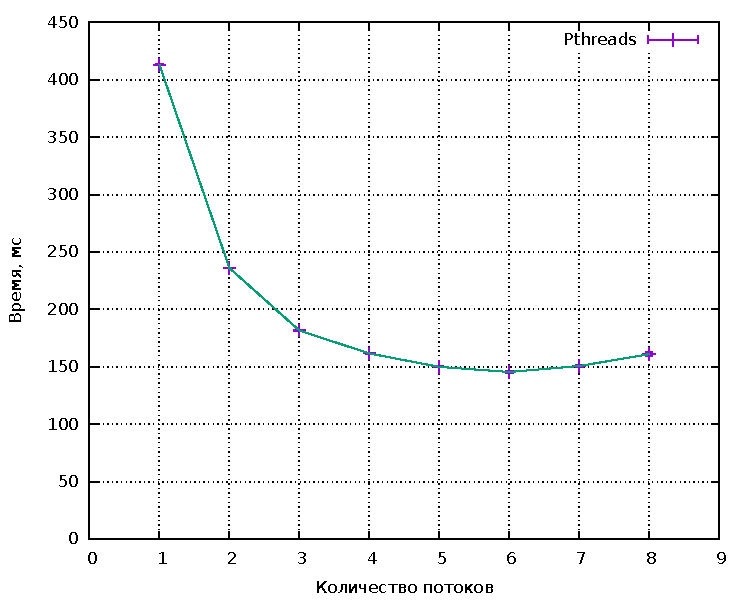
\includegraphics[width=0.8\textwidth]{../plot_gcc/plotPth.pdf}
	\caption{}
\end{figure}

\begin{figure}[H]
	\centering
	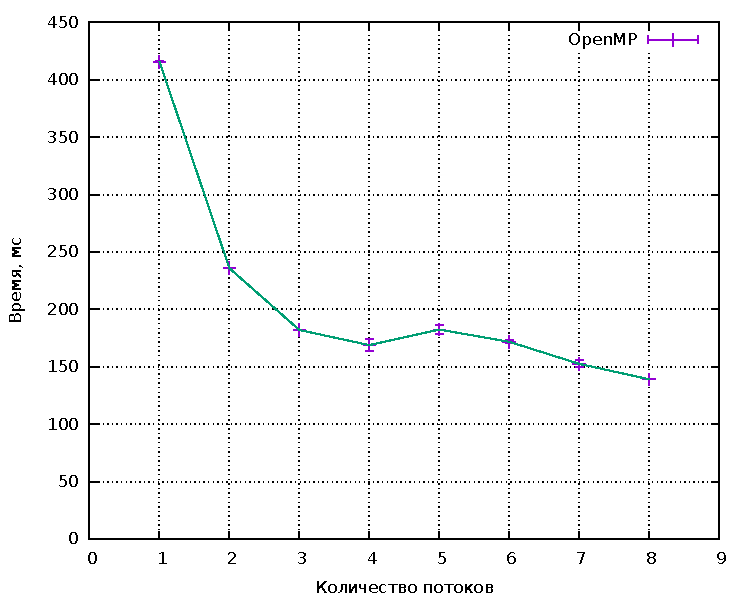
\includegraphics[width=0.8\textwidth]{../plot_gcc/plotMp.pdf}
	\caption{}
\end{figure}

OpenMP:
\begin{verbatim}
Кол-во потоков Время, мс Margin  СКО     Ускорение  
              1    415.70    0.42    2.15       1.00
              2    235.92    0.19    0.95       1.76
              3    182.10    0.20    1.00       2.28
              4    168.89    5.38   27.47       2.46
              5    182.44    4.11   20.98       2.28
              6    171.79    1.39    7.09       2.42
              7    152.63    3.08   15.74       2.72
              8    139.19    0.18    0.93       2.99
\end{verbatim}

Pthreads:
\begin{verbatim}
Кол-во потоков  Время, мс   Margin    СКО     Ускорение  
               1      413.10      0.31    1.57       1.00
               2      236.06      0.17    0.88       1.75
               3      181.63      0.23    1.19       2.27
               4      161.65      0.21    1.08       2.56
               5      149.97      0.38    1.93       2.75
               6      145.56      0.60    3.05       2.84
               7      150.71      1.00    5.11       2.74
               8      161.04      1.85    9.43       2.57
\end{verbatim}

\begin{figure}[H]
	\centering
	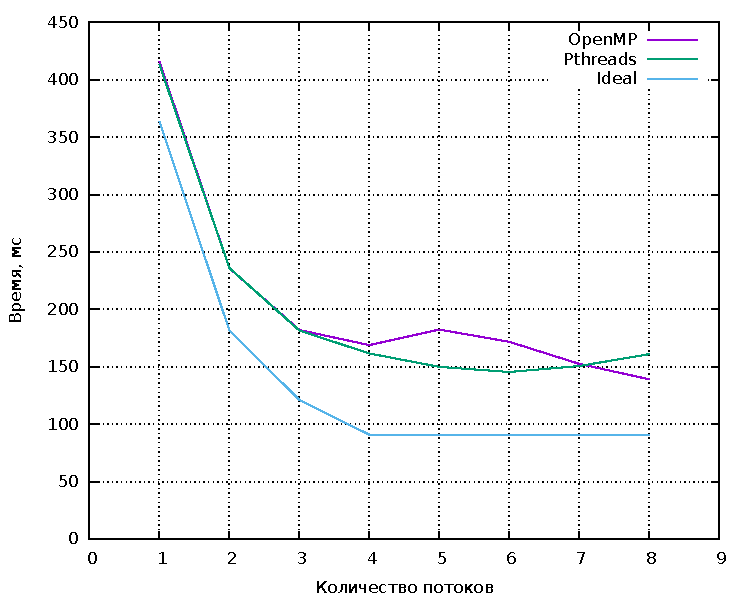
\includegraphics[width=0.8\textwidth]{../plot_gcc/plotAll.pdf}
	\caption{}
\end{figure}

Проведем аналогичный тест, но с использованием компилятора Clang 3.8.

\begin{figure}[H]
	\centering
	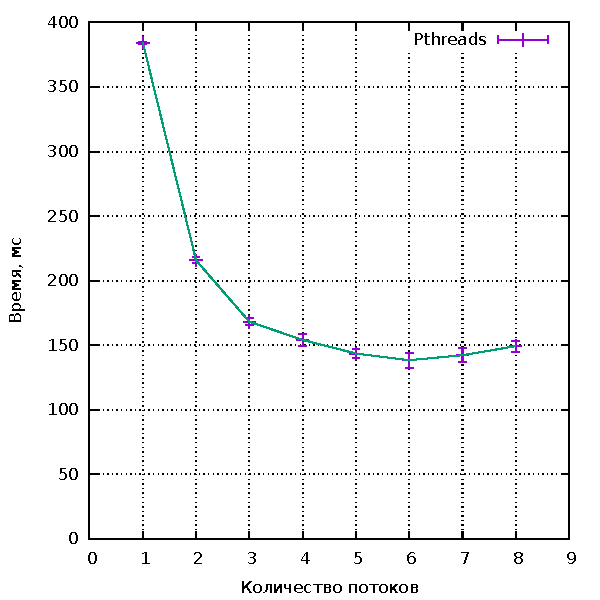
\includegraphics[width=0.8\textwidth]{../plot_clang/plotPth.pdf}
	\caption{}
\end{figure}

\begin{figure}[H]
	\centering
	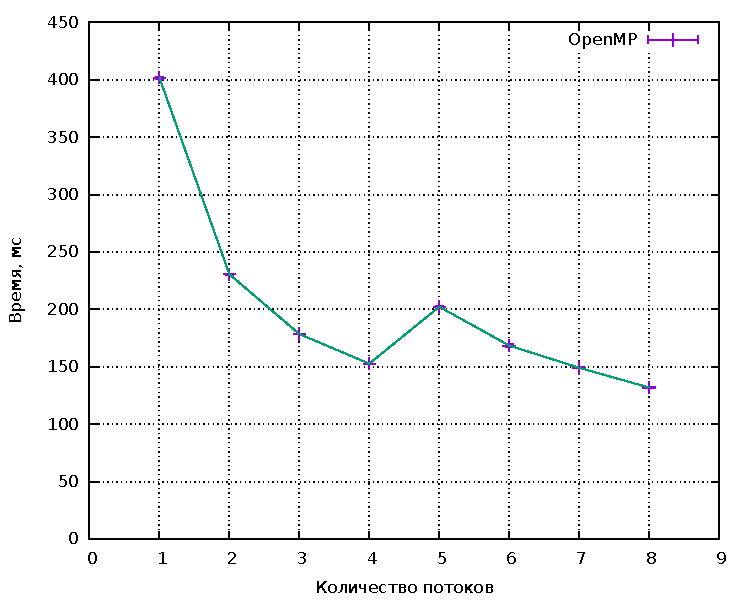
\includegraphics[width=0.8\textwidth]{../plot_clang/plotMp.pdf}
	\caption{}
\end{figure}

\begin{figure}[H]
	\centering
	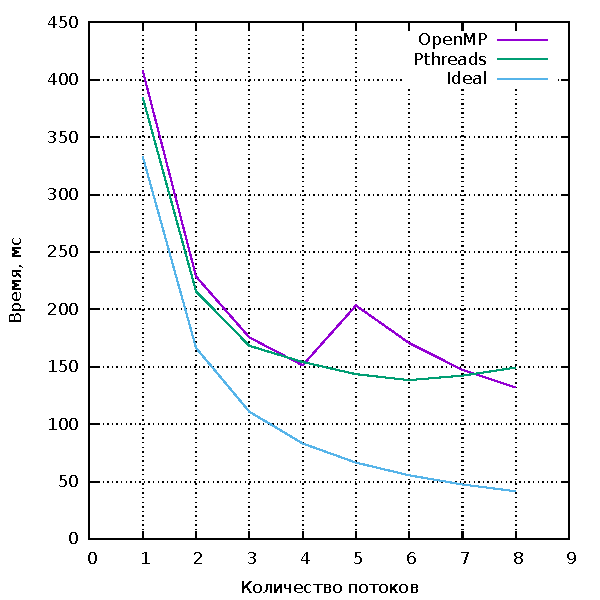
\includegraphics[width=0.8\textwidth]{../plot_clang/plotAll.pdf}
	\caption{}
\end{figure}

По сравнению с GCC немного увеличилась производительность, но соотношения остались примерно теми же.

Тестирование на машине с Core i3 5010u (Broadwell, 2 ядра, 4 потока, 2,1 GHz, одноканальная память DDR3 4 Гб) с аналогичным набором ПО:

\begin{figure}[H]
	\centering
	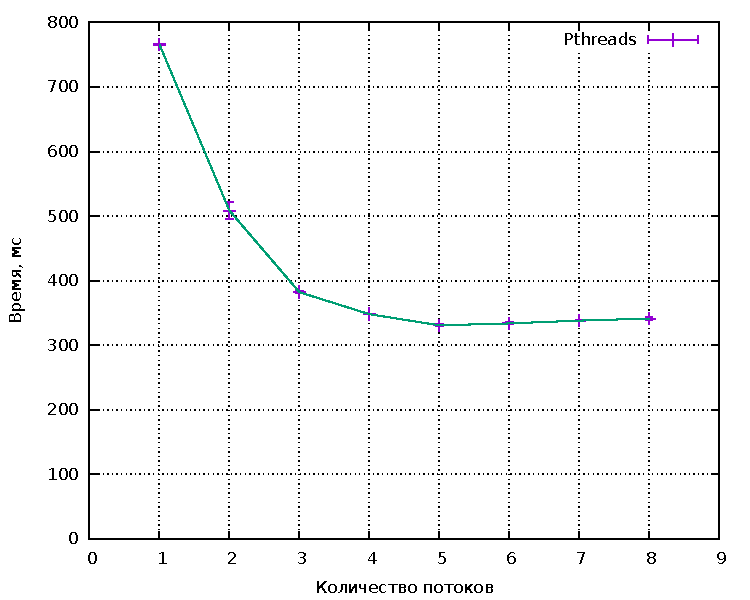
\includegraphics[width=0.8\textwidth]{../plot_laptop/plotPth.pdf}
	\caption{}
\end{figure}

\begin{figure}[H]
	\centering
	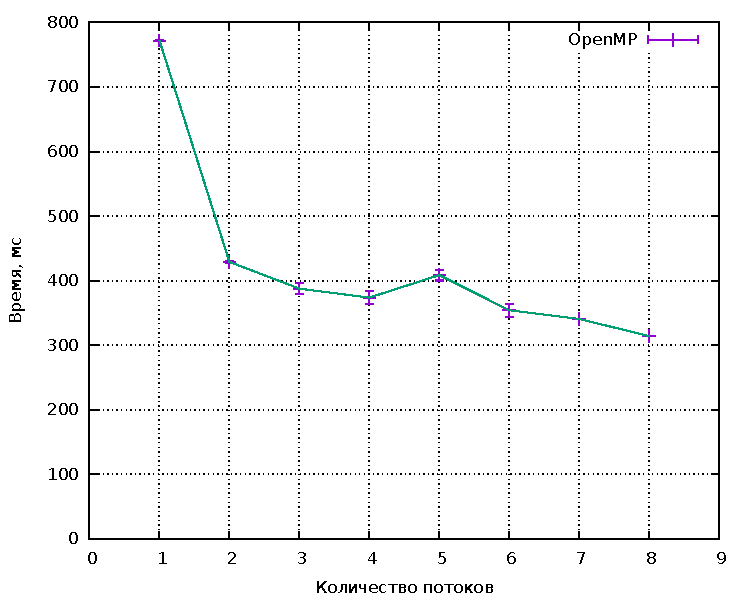
\includegraphics[width=0.8\textwidth]{../plot_laptop/plotMp.pdf}
	\caption{}
\end{figure}

\begin{figure}[H]
	\centering
	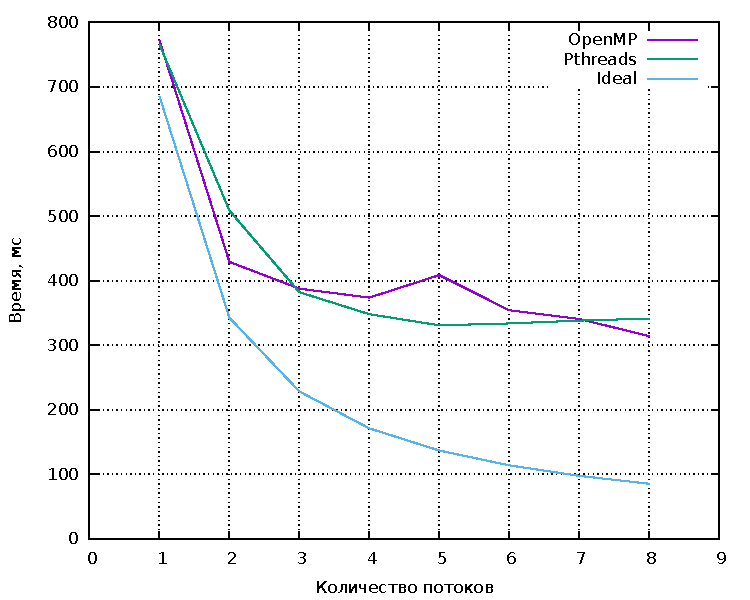
\includegraphics[width=0.8\textwidth]{../plot_laptop/plotAll.pdf}
	\caption{}
\end{figure}

OpenMP:
\begin{verbatim}
Кол-во потоков Время, мс Margin  СКО    Ускорение  
             1    771.91    0.35   1.77       1.00
             2    429.25    1.71   8.72       1.80
             3    387.76    8.80  44.89       1.99
             4    373.89    9.67  49.34       2.06
             5    408.68    8.39  42.79       1.89
             6    354.32    9.85  50.26       2.18
             7    340.76    0.56   2.88       2.27
             8    314.36    0.26   1.33       2.46
\end{verbatim}

Pthreads:
\begin{verbatim}

\end{verbatim}

Что можно заметить:
\begin{itemize}
	\item HyperThreading дает определенные результаты, скорость работы 4 ядер выше, чем 2. Таким образом, удается более эффективно использовать блоки ЦПУ и память.
	\item Производительность i3 в целом меньше в 1,5 раза по сравнению с i5 за счет более низкой частоты.
	\item OpenMP имеет проблемы при 5 потоках. Возможно это связано со сложностями планирования.
	\item При 8 потоках OpenMP быстрее Pthreads. Возможно это связано с тем, что OpenMP использует некоторый пул потоков, а в случае Pthreads потоки создаются каждый раз заново и на это требуется время
\end{itemize}

\section{Выводы}
\begin{itemize}
	\item Основная идея, примененная при решении этой задачи - разбить задачу на несколько частей (блоков), обрабатывать задачи параллельно, а потом объединить результаты
	\item Для предоставление эксклюзивного доступа к разделяемому массиву в OpenMP были использованы критические секции, а в Pthreads - мьютексы.
	\item При увеличении количества потоков производительность растет не линейно - появляются некоторые затраты на синхронизацию. Кроме того, некоторые узлы компьютера (например, интерфейс к памяти) становятся <<бутылочным горлышком>> и препятствуют дальнейшему ускорению. Решение - переход к других архитектурам, например, NUMA, а также переработке программ.
	\item Для правильной оценки производительности нужно использоваться стат. обработку
	\item OpenMP значительно проще в программировании, но допускает меньше контроля и в некоторых ситуациях медленнее
\end{itemize}
